% \section{Jste u nás poprvé?}

% \bigskip
% \subsection{Půjčovna}

% \bigskip
\ifdefined\ikonka\else%
\newcommand\ikonka[1]{\bigskip\bgroup\Large #1\egroup\par}
% \newcommand\ikonka[1]{}
\renewcommand\section[2][]{%
  \bgroup\large \textbf{#2}\egroup\par%
}
\fi
\ikonka{\faPencil}
\section{Fill out the online application form}

% Potřebujete jen průkaz UK (vystavuje ho na~počkání \href{http://www.cuni.cz/UK-3249.html}{\emph{Informační a poradenské
% centrum UK}}). Pak navštivte stránku 
% \textit{knihovna.cuni.cz/e-prihlaska/}.
% \textit{\url{knihovna.cuni.cz/e-prihlaska/}}.
% S touto přihláškou můžete chodit do všech knihoven UK! 

All you need is your Charles University (CU) ID (issued upon request from  
the card service at CU Point). Then visit the following page
to fill out your application form:
library.cuni.cz/e-application/.

After submitting this application form, you will have access to all libraries at Charles University!

\ikonka{\faBook}
\section{Borrowing and returning }

% Většinu knih máme ve skladu, ale připravujeme je obratem.
Most of the books are kept in our storage room, but we prepare them promptly.

% Knihy můžeme nachystat i předem a umístit je do výdejního boxu před studovnou.
% Bez ohledu na naši otevírací dobu si je můžete vyzvednout. Kód k vyzvednutí
% zasíláme SMS zprávou.
We can prepare the books in advance and place them in the pick-up box located
in front of the study room. You can pick up the books at any time, regardless
of our opening hours. We will send you the pick-up code via text message (SMS).


% Standardní výpůjční lhůta je 30 dní a je možné ji prodloužit. K vracení knih
% můžete také využít biblioboxy -- jeden u vrátnice v M. Rettigové 4 a jeden před
% studovnou v Celetné 13.
The standard borrowing period is 30 days and it can be extended. You can also
return the books using the book drops - one is located at the reception desk in
M. Rettigové 4 and the other one is located in front of the study room at
Celetná 13.



\ikonka{\faSearch}
\section{You can find everything in the UKAŽ search engine.}
% \url{ukaz.cuni.cz}

\begin{enumerate}
  % \item Čtenářské konto (přehled výpůjček, možnost jejich prodloužení).

  % \item Veškeré tištěné zdroje. Každý dokument je označen signaturou (např. F54759), podle které knihu snadno vyhledáme.

  % \item Veškeré elektronické zdroje dostupné na UK (e-knihy, e-časopisy, e-články).\\ Jejich přehled najdete na: \textit{knihovna.pedf.cuni.cz/eiz.htm}.
  \item Reader account (overview of loans, possibility of renewal)
  \item All printed resources. Each document is labeled with a call number
    (e.g. F54759), which makes it easy to locate the book.
  \item All electronic resources available at the University of Charles
    (e-books, e-journals, e-articles). You can find the list of available
    resources at knihovna.pedf.cuni.cz/catalogues.html.
\end{enumerate}

\ikonka{\faBed}
\section{Study comfortably from home.}
% Kromě papírových knih a časopisů máme i
% stovky tisíc textů elektronicky.  V~nabídce jsou elektronické
% časopisy, články nebo knihy různých oborů. Jsou dostupné přímo
% z~fakultní sítě nebo pomocí vzdáleného přístupu (s využitím
% přihlašovacích údajů do Centrální autentizační služby).
In addition to paper books and magazines, we also have hundreds of thousands of
electronic texts available. The selection includes electronic journals,
articles, and books from various fields. They are accessible directly from the
university network or through remote access (using login credentials to the
Central Authentication Service).

% Více informací naleznete např. na~\textbf{Portálu elektronických zdrojů
  % {\href{https://ezdroje.cuni.cz}{Univerzity Karlovy}}} nebo ve \textbf{vyhledávači UKAŽ}.
You can find more information, for example, on the Portal of Electronic
Resources of Charles University or in the UKAŽ search engine.

% \ikonka{\faAndroid}
% \section{Help with citations}

% Pokud studujete nebo pracujete na Pedagogické fakultě, můžete bezplatně
% využívat citační manažer Citace PRO. 
% Pokud si s citacemi nevíte rady, rádi pomůžeme.
% Tvořit citace je jednoduché: nechte za sebe pracovat citační manažer.
% Pokud studujete nebo pracujete na~Pedagogické fakultě,
% můžete bezplatně využívat citační manažer Citace PRO.
% Pokud si s citacemi nevíte rady, rádi pomůžeme.

\ikonka{\faInfoCircle}
\section{We advise online and in person} 
% Na dálku poradíme s citováním i rešeršemi přes FB knihovny.

% Zajímá vás, jak efektivně vyhledávat informace, pracovat se zdroji nebo jak
% správně citovat? Ptejte se v naší online poradně přes FB @knihovnapedfpraha,
% nebo nám napište na e-mail. Můžeme si také domluvit osobní konzultace. 
Do you want to know how to search for information efficiently, work with
sources, or cite correctly? Ask us in our online advisory service via FB
@knihovnapedfpraha or write to us via email. We can also arrange personal
consultations.



% \newpage

\ikonka{\faGraduationCap}
\section{Try our study rooms}

% Kromě knih a časopisů tu najdete počítače, tiskárny, kopírky a
% skener. Nabízíme také vázání kroužkovou vazbou. Půjčujeme i notebooky, USB
% nabíječky na telefon, čtečky elektronických knih, deskové hry nebo flash disky. 
In addition to books and journals, you will find computers, printers, copiers,
and scanners here. We also offer spiral binding services. We lend laptops, USB
chargers for phones, e-book readers, board games, or flash drives.

% Pro prezenční studium dokumentů je určena studovna knihovny. 
% Tu mohou využívat studenti s~platným průkazem UK, ale i externí uživatelé. 
% Uloženy jsou zde 
% Ve studovně najdete odborné knihy, odborné i populárně naučné
% časopisy, učebnice, skripta a vždy aktuální denní tisk.

% Využít můžete počítače s přístupem na~internet a do databází,
% samoobslužné tiskárny, kopírky a skener. Nabízíme také vázání kroužkovou vazbou.

% Můžete využít i doplňkových služeb a vypůjčit si 
% Půjčujeme i notebooky, USB nabíječky na
% telefon, čtečky elektronických knih, deskové hry nebo flash disky (vše
% v~rámci studovny).

% \textbf{Máme pro vás týmovou studovnu.} Rezervovat si ji můžete
% vyplněním formuláře na~našem webu. V týmové studovně je k dispozici deset míst
% a tabule na~psaní.
% \textbf{Máme pro vás týmovou studovnu},  kde je k dispozici deset míst
% a tabule na~psaní.
We have \textbf{a team study room} for you with ten seats and a writing board.

% \subsection{Další služby a nástroje}

% \newpage



\bigskip
\ikonka{\faHeart}
\section{Services for students with special needs}

% Studovna je vybavena počítačem s nainstalovaným screen readerem NVDA a Fine
% Readerem. Tento počítač je volně dostupný a je možné ho využívat samostatně.
The study room is equipped with a computer with the NVDA screen reader and Fine
Reader installed. This computer is freely available and can be used
independently.

% Pro studenty se zrakovým znevýhodněním máme k dispozici digitalizované knihy,
% které jsou přístupné z webu knihovny. Na základě registrace obdržíte heslo pro online
% přístup. Tato registrace umožňuje také bezplatný tisk materiálů
% souvisejících se studiem. 

For students with visual impairments, we have digitized books available on the
library's website. Upon registration, you will receive a password for online
access. This registration also allows for the free printing of study-related
materials.

% Studovna je vybavena počítačem s nainstalovaným screen readerem NVDA a Fine
% Readerem. Tento počítač je volně dostupný a je možné ho využívat samostatně.
% Pro studenty se zrakovým znevýhodněním je k dispozici 245 zdigitalizovaných
% knih. Přístupné jsou z webu knihovny. Na základě registrace obdržíte heslo pro
% online přístup k nim. Tato registrace umožňuje také bezplatný tisk materiálů
% souvisejících se studiem. Pro individuální přístup s ohledem k Vašim
% specifickým potřebám nás neváhejte kontaktovat.  

\vfill

\begin{center}

\includegraphics[width=0.5\textwidth]{knihy.png}
\end{center}

\newpage
\section{Where can you find us}

\vskip 1em
\smallsection{Borrowing and Study Room in the main building of the Faculty}

% Těšíme se na~vás v přízemí hlavní budovy Pedagogické fakulty
% na~adrese 
Magdalény Rettigové 4, Prague 1\\
on the ground floor.

% \vskip 3em

\includegraphics[width=\textwidth]{mapka-texty-en.png}

\vskip 1em
\smallsection{Study Room in Celetná}

Celetná 13, Prague 1, in the attic.

\begin{center}

\includegraphics[width=0.4\textwidth]{schody.png}
\end{center}


% \textbf{Jak se k~nám dostanete?}

% \begin{itemize}[leftmargin=0pt, topsep=0pt]
% \item
%   metrem B, stanice Národní třída -- výtahem přímo do ulice Magdalény
%   Rettigové
% \item
%   tramvají č. 3, 6, 9, 14, 24 zastávka Lazarská
% \end{itemize}

% \smallsection{Knihovna je rozdělena na dvě části:}

% \begin{itemize}[leftmargin=0pt, topsep=0pt]
% \item Půjčovna se nachází napravo od hlavního vchodu
%   do budovy, přes dvorek, vedle zadního vchodu do Auly.
% \item Studovna  je na levé straně budovy.
% \end{itemize}

  % \rotatebox{90}{% Graphic for TeX using PGF
% Title: /home/mint/knihovna/planekknihovny.dia
% Creator: Dia v0.97.3
% CreationDate: Tue Oct 10 14:49:24 2017
% For: mint
% \usepackage{tikz}
% The following commands are not supported in PSTricks at present
% We define them conditionally, so when they are implemented,
% this pgf file will use them.
\ifx\du\undefined
  \newlength{\du}
\fi
\setlength{\du}{11\unitlength}
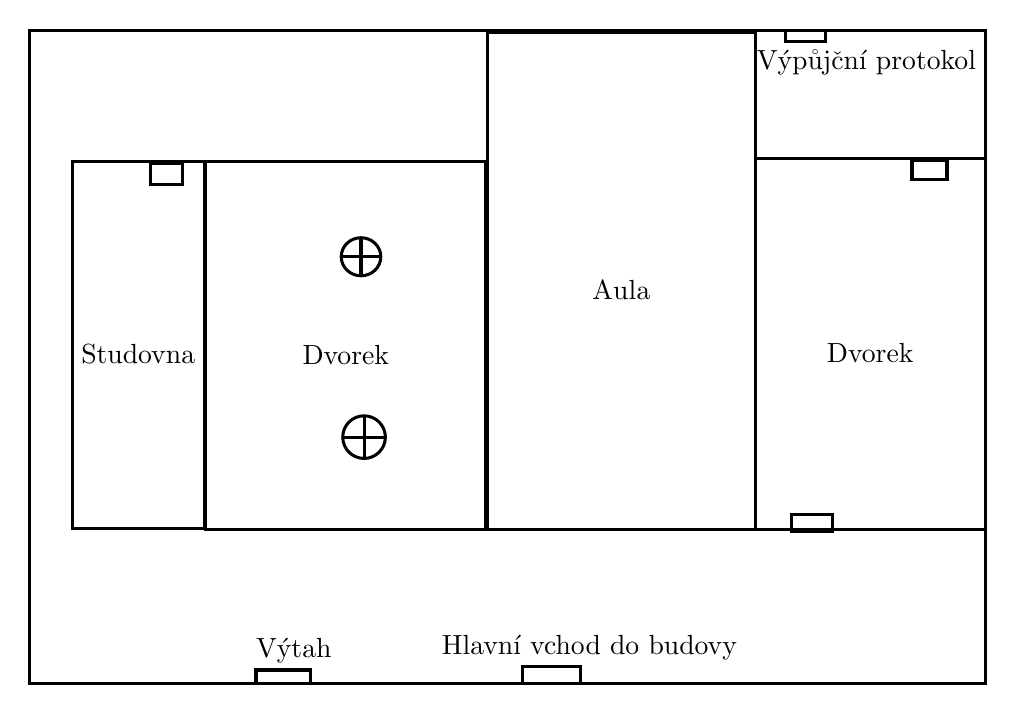
\begin{tikzpicture}
\pgftransformxscale{1.000000}
\pgftransformyscale{-1.000000}
\definecolor{dialinecolor}{rgb}{0.000000, 0.000000, 0.000000}
\pgfsetstrokecolor{dialinecolor}
\definecolor{dialinecolor}{rgb}{1.000000, 1.000000, 1.000000}
\pgfsetfillcolor{dialinecolor}
\definecolor{dialinecolor}{rgb}{1.000000, 1.000000, 1.000000}
\pgfsetfillcolor{dialinecolor}
\fill (0.300000\du,4.300000\du)--(0.300000\du,25.750000\du)--(31.700000\du,25.750000\du)--(31.700000\du,4.300000\du)--cycle;
\pgfsetlinewidth{0.100000\du}
\pgfsetdash{}{0pt}
\pgfsetdash{}{0pt}
\pgfsetmiterjoin
\definecolor{dialinecolor}{rgb}{0.000000, 0.000000, 0.000000}
\pgfsetstrokecolor{dialinecolor}
\draw (0.300000\du,4.300000\du)--(0.300000\du,25.750000\du)--(31.700000\du,25.750000\du)--(31.700000\du,4.300000\du)--cycle;
% setfont left to latex
\definecolor{dialinecolor}{rgb}{0.000000, 0.000000, 0.000000}
\pgfsetstrokecolor{dialinecolor}
\node at (16.000000\du,15.310000\du){};
\definecolor{dialinecolor}{rgb}{1.000000, 1.000000, 1.000000}
\pgfsetfillcolor{dialinecolor}
\fill (6.100000\du,8.600000\du)--(6.100000\du,20.700000\du)--(15.300000\du,20.700000\du)--(15.300000\du,8.600000\du)--cycle;
\pgfsetlinewidth{0.100000\du}
\pgfsetdash{}{0pt}
\pgfsetdash{}{0pt}
\pgfsetmiterjoin
\definecolor{dialinecolor}{rgb}{0.000000, 0.000000, 0.000000}
\pgfsetstrokecolor{dialinecolor}
\draw (6.100000\du,8.600000\du)--(6.100000\du,20.700000\du)--(15.300000\du,20.700000\du)--(15.300000\du,8.600000\du)--cycle;
% setfont left to latex
\definecolor{dialinecolor}{rgb}{0.000000, 0.000000, 0.000000}
\pgfsetstrokecolor{dialinecolor}
\node at (10.700000\du,14.935000\du){Dvorek};
\definecolor{dialinecolor}{rgb}{1.000000, 1.000000, 1.000000}
\pgfsetfillcolor{dialinecolor}
\fill (15.350000\du,4.350000\du)--(15.350000\du,20.700000\du)--(24.150000\du,20.700000\du)--(24.150000\du,4.350000\du)--cycle;
\pgfsetlinewidth{0.100000\du}
\pgfsetdash{}{0pt}
\pgfsetdash{}{0pt}
\pgfsetmiterjoin
\definecolor{dialinecolor}{rgb}{0.000000, 0.000000, 0.000000}
\pgfsetstrokecolor{dialinecolor}
\draw (15.350000\du,4.350000\du)--(15.350000\du,20.700000\du)--(24.150000\du,20.700000\du)--(24.150000\du,4.350000\du)--cycle;
% setfont left to latex
\definecolor{dialinecolor}{rgb}{0.000000, 0.000000, 0.000000}
\pgfsetstrokecolor{dialinecolor}
\node at (19.750000\du,12.810000\du){Aula};
\pgfsetlinewidth{0.100000\du}
\pgfsetdash{}{0pt}
\pgfsetdash{}{0pt}
\pgfsetbuttcap
\pgfsetmiterjoin
\pgfsetlinewidth{0.100000\du}
\pgfsetbuttcap
\pgfsetmiterjoin
\pgfsetdash{}{0pt}
\definecolor{dialinecolor}{rgb}{1.000000, 1.000000, 1.000000}
\pgfsetfillcolor{dialinecolor}
\pgfpathellipse{\pgfpoint{11.300000\du}{17.650000\du}}{\pgfpoint{0.700000\du}{0\du}}{\pgfpoint{0\du}{0.700000\du}}
\pgfusepath{fill}
\definecolor{dialinecolor}{rgb}{0.000000, 0.000000, 0.000000}
\pgfsetstrokecolor{dialinecolor}
\pgfpathellipse{\pgfpoint{11.300000\du}{17.650000\du}}{\pgfpoint{0.700000\du}{0\du}}{\pgfpoint{0\du}{0.700000\du}}
\pgfusepath{stroke}
\pgfsetbuttcap
\pgfsetmiterjoin
\pgfsetdash{}{0pt}
\definecolor{dialinecolor}{rgb}{0.000000, 0.000000, 0.000000}
\pgfsetstrokecolor{dialinecolor}
\draw (11.300000\du,16.950000\du)--(11.300000\du,18.350000\du);
\pgfsetbuttcap
\pgfsetmiterjoin
\pgfsetdash{}{0pt}
\definecolor{dialinecolor}{rgb}{0.000000, 0.000000, 0.000000}
\pgfsetstrokecolor{dialinecolor}
\draw (10.600000\du,17.650000\du)--(12.000000\du,17.650000\du);
\pgfsetlinewidth{0.100000\du}
\pgfsetdash{}{0pt}
\pgfsetdash{}{0pt}
\pgfsetbuttcap
\pgfsetmiterjoin
\pgfsetlinewidth{0.100000\du}
\pgfsetbuttcap
\pgfsetmiterjoin
\pgfsetdash{}{0pt}
\definecolor{dialinecolor}{rgb}{1.000000, 1.000000, 1.000000}
\pgfsetfillcolor{dialinecolor}
\pgfpathellipse{\pgfpoint{11.200000\du}{11.725000\du}}{\pgfpoint{0.650000\du}{0\du}}{\pgfpoint{0\du}{0.625000\du}}
\pgfusepath{fill}
\definecolor{dialinecolor}{rgb}{0.000000, 0.000000, 0.000000}
\pgfsetstrokecolor{dialinecolor}
\pgfpathellipse{\pgfpoint{11.200000\du}{11.725000\du}}{\pgfpoint{0.650000\du}{0\du}}{\pgfpoint{0\du}{0.625000\du}}
\pgfusepath{stroke}
\pgfsetbuttcap
\pgfsetmiterjoin
\pgfsetdash{}{0pt}
\definecolor{dialinecolor}{rgb}{0.000000, 0.000000, 0.000000}
\pgfsetstrokecolor{dialinecolor}
\draw (11.200000\du,11.100000\du)--(11.200000\du,12.350000\du);
\pgfsetbuttcap
\pgfsetmiterjoin
\pgfsetdash{}{0pt}
\definecolor{dialinecolor}{rgb}{0.000000, 0.000000, 0.000000}
\pgfsetstrokecolor{dialinecolor}
\draw (10.550000\du,11.725000\du)--(11.850000\du,11.725000\du);
\definecolor{dialinecolor}{rgb}{1.000000, 1.000000, 1.000000}
\pgfsetfillcolor{dialinecolor}
\fill (24.153750\du,8.500000\du)--(24.153750\du,20.700000\du)--(31.700000\du,20.700000\du)--(31.700000\du,8.500000\du)--cycle;
\pgfsetlinewidth{0.100000\du}
\pgfsetdash{}{0pt}
\pgfsetdash{}{0pt}
\pgfsetmiterjoin
\definecolor{dialinecolor}{rgb}{0.000000, 0.000000, 0.000000}
\pgfsetstrokecolor{dialinecolor}
\draw (24.153750\du,8.500000\du)--(24.153750\du,20.700000\du)--(31.700000\du,20.700000\du)--(31.700000\du,8.500000\du)--cycle;
% setfont left to latex
\definecolor{dialinecolor}{rgb}{0.000000, 0.000000, 0.000000}
\pgfsetstrokecolor{dialinecolor}
\node at (27.926875\du,14.885000\du){Dvorek};
\definecolor{dialinecolor}{rgb}{1.000000, 1.000000, 1.000000}
\pgfsetfillcolor{dialinecolor}
\fill (1.707500\du,8.600000\du)--(1.707500\du,20.650000\du)--(6.050000\du,20.650000\du)--(6.050000\du,8.600000\du)--cycle;
\pgfsetlinewidth{0.100000\du}
\pgfsetdash{}{0pt}
\pgfsetdash{}{0pt}
\pgfsetmiterjoin
\definecolor{dialinecolor}{rgb}{0.000000, 0.000000, 0.000000}
\pgfsetstrokecolor{dialinecolor}
\draw (1.707500\du,8.600000\du)--(1.707500\du,20.650000\du)--(6.050000\du,20.650000\du)--(6.050000\du,8.600000\du)--cycle;
% setfont left to latex
\definecolor{dialinecolor}{rgb}{0.000000, 0.000000, 0.000000}
\pgfsetstrokecolor{dialinecolor}
\node at (3.878750\du,14.910000\du){Studovna};
\pgfsetlinewidth{0.100000\du}
\pgfsetdash{}{0pt}
\pgfsetdash{}{0pt}
\pgfsetmiterjoin
\definecolor{dialinecolor}{rgb}{1.000000, 1.000000, 1.000000}
\pgfsetfillcolor{dialinecolor}
\fill (25.350000\du,20.200000\du)--(25.350000\du,20.350000\du)--(26.700000\du,20.350000\du)--(26.700000\du,20.200000\du)--cycle;
\definecolor{dialinecolor}{rgb}{0.000000, 0.000000, 0.000000}
\pgfsetstrokecolor{dialinecolor}
\draw (25.350000\du,20.200000\du)--(25.350000\du,20.750000\du)--(26.700000\du,20.750000\du)--(26.700000\du,20.200000\du)--cycle;
\pgfsetlinewidth{0.100000\du}
\pgfsetdash{}{0pt}
\pgfsetdash{}{0pt}
\pgfsetmiterjoin
\definecolor{dialinecolor}{rgb}{1.000000, 1.000000, 1.000000}
\pgfsetfillcolor{dialinecolor}
\fill (29.300000\du,8.550000\du)--(29.300000\du,9.200000\du)--(30.450000\du,9.200000\du)--(30.450000\du,8.550000\du)--cycle;
\definecolor{dialinecolor}{rgb}{0.000000, 0.000000, 0.000000}
\pgfsetstrokecolor{dialinecolor}
\draw (29.300000\du,8.550000\du)--(29.300000\du,9.200000\du)--(30.450000\du,9.200000\du)--(30.450000\du,8.550000\du)--cycle;
\pgfsetlinewidth{0.100000\du}
\pgfsetdash{}{0pt}
\pgfsetdash{}{0pt}
\pgfsetmiterjoin
\definecolor{dialinecolor}{rgb}{1.000000, 1.000000, 1.000000}
\pgfsetfillcolor{dialinecolor}
\fill (25.150000\du,4.200000\du)--(25.150000\du,4.650000\du)--(26.450000\du,4.650000\du)--(26.450000\du,4.200000\du)--cycle;
\definecolor{dialinecolor}{rgb}{0.000000, 0.000000, 0.000000}
\pgfsetstrokecolor{dialinecolor}
\draw (25.150000\du,4.300000\du)--(25.150000\du,4.650000\du)--(26.450000\du,4.650000\du)--(26.450000\du,4.300000\du)--cycle;
\pgfsetlinewidth{0.100000\du}
\pgfsetdash{}{0pt}
\pgfsetdash{}{0pt}
\pgfsetmiterjoin
\definecolor{dialinecolor}{rgb}{1.000000, 1.000000, 1.000000}
\pgfsetfillcolor{dialinecolor}
\fill (4.300000\du,8.650000\du)--(4.300000\du,9.350000\du)--(5.350000\du,9.350000\du)--(5.350000\du,8.650000\du)--cycle;
\definecolor{dialinecolor}{rgb}{0.000000, 0.000000, 0.000000}
\pgfsetstrokecolor{dialinecolor}
\draw (4.300000\du,8.650000\du)--(4.300000\du,9.350000\du)--(5.350000\du,9.350000\du)--(5.350000\du,8.650000\du)--cycle;
\pgfsetlinewidth{0.100000\du}
\pgfsetdash{}{0pt}
\pgfsetdash{}{0pt}
\pgfsetmiterjoin
\definecolor{dialinecolor}{rgb}{1.000000, 1.000000, 1.000000}
\pgfsetfillcolor{dialinecolor}
\fill (16.500000\du,25.200000\du)--(16.500000\du,25.750000\du)--(18.400000\du,25.750000\du)--(18.400000\du,25.200000\du)--cycle;
\definecolor{dialinecolor}{rgb}{0.000000, 0.000000, 0.000000}
\pgfsetstrokecolor{dialinecolor}
\draw (16.500000\du,25.200000\du)--(16.500000\du,25.750000\du)--(18.400000\du,25.750000\du)--(18.400000\du,25.200000\du)--cycle;
% setfont left to latex
\definecolor{dialinecolor}{rgb}{0.000000, 0.000000, 0.000000}
\pgfsetstrokecolor{dialinecolor}
\node[anchor=west] at (16.000000\du,15.025000\du){};
% setfont left to latex
\definecolor{dialinecolor}{rgb}{0.000000, 0.000000, 0.000000}
\pgfsetstrokecolor{dialinecolor}
\node[anchor=west] at (23.850000\du,5.350000\du){Výpůjční protokol};
% setfont left to latex
\definecolor{dialinecolor}{rgb}{0.000000, 0.000000, 0.000000}
\pgfsetstrokecolor{dialinecolor}
\node[anchor=west] at (13.500000\du,24.550000\du){Hlavní vchod do budovy};
\pgfsetlinewidth{0.100000\du}
\pgfsetdash{}{0pt}
\pgfsetdash{}{0pt}
\pgfsetmiterjoin
\definecolor{dialinecolor}{rgb}{1.000000, 1.000000, 1.000000}
\pgfsetfillcolor{dialinecolor}
\fill (7.750000\du,25.300000\du)--(7.750000\du,25.650000\du)--(9.550000\du,25.650000\du)--(9.550000\du,25.300000\du)--cycle;
\definecolor{dialinecolor}{rgb}{0.000000, 0.000000, 0.000000}
\pgfsetstrokecolor{dialinecolor}
\draw (7.750000\du,25.300000\du)--(7.750000\du,25.750000\du)--(9.550000\du,25.750000\du)--(9.550000\du,25.300000\du)--cycle;
% setfont left to latex
\definecolor{dialinecolor}{rgb}{0.000000, 0.000000, 0.000000}
\pgfsetstrokecolor{dialinecolor}
\node[anchor=west] at (7.400000\du,24.650000\du){Výtah};
\end{tikzpicture}
}

\vskip 2em
\section{Contacts}

\begin{tabular}{@{}ll@{}}
  E-mail:& \url{knihovna@pedf.cuni.cz}\\

  Borrowing service:& 221\,900\,148\\
  Study Room:& 221\,900\,178\\
  Study Room Celetná:& 221\,900\,759\\
  Facebook: & \url{@knihovnapedfpraha}\\
  Instagram: & \url{@knihovnapedfpraha}
\end{tabular}

% \newpage
  % \newpage
\vskip 1em
\section{Opening Hours}

\smallsection{Borrowing Room in M. Rettigové}

\begin{tabular}{@{}ll}
  Mo--Fri & 9:00 -- 17:00\\
\end{tabular}


\vskip 1em
\noindent\smallsection{Study Room in M. Retttigové}

\begin{tabular}{@{}ll}
  Mo--Thu &  8:00 -- 18:00\\
  Fri & 8:00 -- 17:00\\
\end{tabular}

\vskip 1em
\noindent\smallsection{Study Room Celetná}

\begin{tabular}{@{}lr}
  Mo &  13:00  -- 18:00\\
  Tue &   9:00  -- 18:00\\
  Wed &   9:00  -- 18:00\\
  Thu &   9:00  -- 18:00\\
  Fri &   9:00  -- 13:00\\
  % Po &  10.00 -- 15.30\\
  % St & 9.00 -- 18.00\\
\end{tabular}
\vskip 2em
\section{Links}

\footnotesize
\begin{tabular}{@{}ll@{}}
  Library:& \url{knihovna.pedf.cuni.cz} \\

  The UKAŽ search engine:& \url{ukaz.cuni.cz} \\
  % Centrální autentizační služba:& \url{cas.cuni.cz}\\
  Portal of Electronic Resources:& \url{ezdroje.cuni.cz}\\
  % Citace PRO: & \url{citace.com/citace-pro} \\
  % Vyřazené knihy -- e-shop &\url{knihovna.pedf.cuni.cz/wp/} \\

  % Ústřední knihovna UK:& \url{knihovna.cuni.cz} \\

  % IPSC UK:& \url{ipc.cuni.cz} 
\end{tabular}
% \newpage
